\documentclass[12pt,a4paper]{report}
\usepackage[utf8]{inputenc}
\usepackage{graphicx}
\usepackage{wrapfig}

\renewcommand{\chaptername}{}

\title{
Final Report - ESCiMO \\
in \LaTeX{}
}

\author{
Joris Vergeer - 1585591\\
Gerben Boot - 1575754\\
\\
\\
Daniel Telgren
}

\begin{document}
\maketitle

\begin{abstract}
%%
%%TODO Rewrite parts of this
%%
Grid Manufacturing (GM) is a new production paradigm, based upon the use of standardized and modular Reconfigurable Manufacturing Systems (RMS).\cite{SICE13}
A production unit in a RMS is called an equiplet.
Each equiplet contains interchangeable modules. 
These hardware modules have software counterparts.
In this report we look at the realisation of the state machines build into the software counterparts of modules and equiplets as well as the realisation of a SCADA for the equiplet with its modules.
\end{abstract}

\tableofcontents


\chapter{Introduction}
In the 6th semester of our course Computer Science at the University of Applied Science Utrecht we participated in the Ubiquitous Computing specialisation.

\section{Agile/Grid manufacturing}
To meet the requirements of modern production, where short
time to market, requirement-driven production and low cost
small quantity production are important issues, we have de-
veloped a production hardware infrastructure as well as an
agent-based software infrastructure for agile industrial pro-
duction. This production is done on special devices called
equiplets. A grid of these equiplets connected by a fast net-
work is capable of producing a variety of different products
in parallel. The multi-agent-based software infrastructure is
responsible for the agile manufacturing.\cite{Paper70}

\section{Equiplet}
The Equiplet is a part of the Agile/Grid manufacturing. The Agent consist of multiple agents and controls one or more modules. Based on the connected modules of the equiplet, provide the equiplet services for an other agent in the Agile/Grid manufactoring environment. 
\subsection{Equiplet Agent}
The equiplet agent is the leading agent for the equiplet. It is responsible for negotiation with the product agent and managing the equiplet schedule.\cite{REXOS_Design}
\subsection{Service Agent}
The service agent is responsible for translating a product step into service step(s). The service agent also represents equiplet services based on the attached modules. The set of product steps which can be performed is based on the services it provides.\cite{REXOS_Design}
\subsection{Hardware Agent}
The hardware agent is responsible for the interaction with the ROS layer. It translates service steps into equiplet steps, which can be interpreted by the ROS layer. It has a specific piece of software for each hardware module that is currently attached to the equiplet. Each one of these pieces of software is responsible for its own hardware module on the equiplet, and handle the actual translation. Each service step has a specific module that will lead the translation. \cite{REXOS_Design}
\subsection{ROS Equiplet}
The ros equiplet is the responsible for the control of a set of modules which belong to by the equiplet. This equiplet part works with the the ROS system.

\section{Module}
An module is an part of the system which controls one or more devices. This part can be seen as the lowest layer of the hardware control.
There are actor and no-actor modules. The actor modules are the modules which is an risk for an human if he is close to the module. The no-actors can be seen as the sensor modules which produce measured information.  

\section{Blackboards}
The Agile Manufacturing contain of three blackboard:Product steps,Service steps and Equiplet steps. These blackboard will be used to communicate between the equiplet agents or to communicate with the ROS node. All these blackboard steps contain a state, about the progress of the step:EVALUATING, PLANNED, WAITING, IN PROGRESS, SUSPENDED/WARNING, DONE, ABORTED and FAILED.

\section{State Machine}
A finite-state machine (FSM) or finite-state automaton (plural: automata), or simply a state machine, is a mathematical model of computation used to design both computer programs and sequential logic circuits. It is conceived as an abstract machine that can be in one of a finite number of states. The machine is in only one state at a time; the state it is in at any given time is called the current state. It can change from one state to another when initiated by a triggering event or condition; this is called a transition. A particular FSM is defined by a list of its states, and the triggering condition for each transition.\cite{state_machine}
\subsection{Why must we used it}
\subsubsection{Safety}
Equiplets are autonomous machines. 
They are part of a large production platform where multiple entities can request actions form the equiplet.
These requests can be received at any time.
Even when an operator is working on an equiplet.
When an operator is working on an equiplet, it has to be absolutely safe.
Modules must be powered off and have to be guarantee that they will not power up while the operator is still nearby.
To prevent this a safety mechanism has to be build.
\subsubsection{Synchronisation}
When instructions require actions from multiple modules both modules have to be ready.
Modules are not guaranteed to be ready at the same time. Some modules require initialisation  and/or calibration procedures while other modules are immediately ready.
To prevent instructions to be send to modules which are not ready yet a synchronisation mechanism has to be build
\subsection{MAST}
\begin{wrapfigure}{r}{0.35\textwidth}
	\begin{center}
		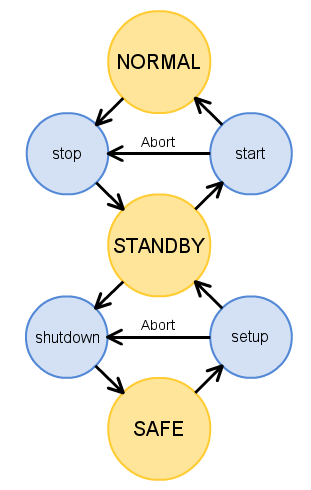
\includegraphics[scale=0.5]{mast.png}
	\caption{MAST}
	\end{center}
	\vspace{-100pt}
\end{wrapfigure}
MAST is a State Machine which is developed for the Agile/Grid Manufacturing project. MAST is designed for the modules to control its devices. Mast implemented three states and four transition states.
\subsubsection{States}
The state machine will have three states:
\begin{itemize}
\item \textbf{Safe} This will mean safe for an human and no power on the machine.
\item \textbf{Standby} This will mean the module will be ready to run, but isn’t running.
\item \textbf{Normal} This will mean the module is in progress.
\end{itemize}
\subsubsection{Transition states}
Between the states there are transition states, which is the only way to change from state. Transition states are responsible to set the machine correct to the next state according the state requirements.  
There are four transition states.
\paragraph{Setup to change from safe to standby}
Set up the module such as calibrating etc.
\paragraph{Shutdown to change from standby to safe}
Shutdown the module
\paragraph{Start to change from standby to normal}The module is receive run information
\paragraph{Stop to change from normal to standby}The module is stopping operations.
\paragraph{Abort}
It will be possible that in a transition state the transition will be undo. This is possible by a ‘abort’. When the machine in a transition state and the transition must be aborted, the transition must stop its commands and change from state to its contrary state. 
The next aborts are possible: from 'setup to shutdown' and from 'start to stop'. 
\subsubsection{Actors and nonactors}
A distinction is made between modules that contain parts that are potentially dangerous and modules that do not contain these parts. These parts are, amongst others, all moving parts,parts that heat up, parts that eject matter and parts that emit electromagnetic radiation. Modules that contain any of these parts are known as actors. Their counterparts (modules that are not potentially dangerous) are nonactors.\cite{mast_funcional_design}
\subsection{The equiplet states}
Due to the nature of the (autonomous) modules in the reconfigurable system the modules can have states that differ from one another. The equiplet node is the central point in which all modules are known. The equiplet itself has two states, one to monitor safety and one to monitor operation. Each state depends on the states of the modules attached to the equiplet in its own
way.
\textbf{The safety state} indicates the level of safety and is equal to the highest actor module state.
\textbf{The operation state} indicates whether the equiplet is able to fulfill the current task and is equal to the lowest state of the required modules. The required modules are the modules necessary tofulfill the current task as known by the hardware agent.\cite{mast_funcional_design}

\section{Equiplet, SCada, MOdules (ESCiMO)}
In our ubiquitous computing project we are developing a system to control a production unit in an RMS called equiplet. 

Equiplets contain interchangeable modules. 
You can reconfigure an equiplet by changing its modules.
Because modules can be changed on the fly, the equiplet has to dynamically adapt to its new configuration.
Due to the autonomous nature of equiplets they can receive instruction at any time.

This together creates a lot of problems we have to solve.


\chapter{Project team}
The following people have worked on ESCiMO

\begin{tabular}{l | l}
Name       & Role \\
\hline
D. Telgren & Project supervisor \\
G. Boot    & Software developer EST, MOST \\
J. Vergeer & Software developer SCADA, MOST
\end{tabular}


\chapter{Assignment}

\section{Problem description}
\subsection{State Machine}
The current State Machine MAST which the Modules implemented miss some required functionality. These missing have been described here.
\subsubsection{Emergency button}
A module has always an emergency button to guarantees safety. When the emergency button is pressed, the software must react on it.
\subsubsection{Errors}
Modules can break down during operation. When this happens it should not receive more tasks from the equiplet to execute. Also its current tasks can not finish.
\subsubsection{(Re-)configuration}
The current state-machine hasn't options to switch to an position to (re-)configurate or to switch to a mode of repair. An repair would see more technical information about the hardware executions and want to reconfigure.
\subsubsection{Lock}
A human would the option to lock on a state of the state machine such as to lock on safe or standby. Lock will means that it isn't possible to call transitions. When the human lock on safe, it guarantees that the state machine hold the safe position.
\subsection{Equiplet control}
The equiplet controls one or more modules. All modules implement a State Machine, but the equiplet must react on changes of the State Machine of the modules.
\subsubsection{Error Handling}
When a module in error, the equiplet should to stop executing its current equiplet step and set it on an aborted state. This option is possible, because all blackboard steps contains states. 
\\Also when a module in error there are two options:
\begin{enumerate}
\item Stop executing equiplet steps
\item Stop executing equiplet steps which needed the module which in error.
\end{enumerate}
In both cases, the equiplet must react when a module in error.
\subsubsection{Step control}
Some equiplet has a (mostly)yellow button. This button should be needed to execute equiplet steps by once and execute next by a press on the button.
\subsection{SCADA}
To operate an equiplet the operator has to be able to see what is going on with the equiplet and modules. He also want an interface where he can perform minimal interaction with the equiplet. Therefore also a SCADA system has to be developed.

\section{Goals}
\begin{itemize}
\item Redesign State Machine
\item Design equiplet State Machine control
\item Design SCADA of the equiplet
\item Implement designed functionality
\end{itemize}

\section{Requirements and conditions}
\subsection{Module State Machine}
\subsubsection{Modes}
Mode is an additional of the State Machine to implement the missing elements described at chapter 3.1.1.
Currently the State Machine contains of states and transitions. A mode is an new dimension at the State Machine. In this case the State Machine react depended on its state and also on its mode.
\paragraph{Emergency Stop}In this mode the modules has lost the devices control and it is possible to show the State Machine as safe.
\paragraph{Error Mode}The error is intended for non-actor modules which in error. The State Machine may not allowed to startup. When a module in error and the State Machine in Normal, the module must try to finish it task and go to standby by stop.
\paragraph{Critical Error Mode}The Critical error mode is intended for actor modules which in error. When an actor module in error, the module should stop when in normal and shutdown when in standby.
\paragraph{Service}The Service mode will be used to add configuration calls to the module. In this mode the repairer should be used this calls.
 
\subsection{Equiplet State Machine control}
\subsubsection{Emergency Stop}
When the emergency button is pressed, the equiplet can't execute equiplet steps, because the hardware of the modules are offline.
\subsubsection{Module in Error}
When a module in error (this means a non-actor module) the other modules must try to finish its task if running. It is possible to run new tasks without the module which in error, but this is not usual said by Erik Puik. He prefer that an equiplet only runs tasks which use all its modules, so the equiplet will always full use its components(modules) and is attractive to the market. In this case we can say when an module in error, the equiplet is also in error.
\subsubsection{Module in Critical Error}
When a module in critical error (this means a actor module) the other modules must abort its task and stop/shutdown. In this case an actor module constitutes a risk so the modules of the equiplet must shutdown to safe.

\subsection{Equiplet opportunities}
\subsubsection{Step control}
The equiplet should execute exeplet steps by once named as 'Step control'.

\section{Final products}
\subsection{State Machine}
Our first product is a state machine for modules and equiplets. 

In addition to states, there are also modes.
A mode defines which states and transitions are allowed.

\subsubsection{MOdule STatemachine (MOST)}
The module state machine is an expansion of MAST with modes.
The state machine is our solution for the error handling, safety guarantee and synchronisation.

\subsubsection{Equiplet STatemachine (EST)}
The EST variant of the state machine is implemented in the equiplet.
It has additional functionality for managing registered MOST state machines and also include modes.

\subsection{SCADA}
The SCADA gives operators insight into the equiplet.
It shows the current state and modes of the equiplet and its modules.
It also gives the operator some control over the equiplet.
In the SCADA he can change the mode and state of the equiplet and its modules.

\subsection{Implementation}
Finally we will implement the state machines in existing modules and equiplets.

\subsection{Documentation}
\paragraph{Project Transfer Document}We also make a Project Transfer Document with the parts of our design and describe what is done and what remains to be done.

\chapter{Analysis}
\section{Overview}

\section{Analysis}

\chapter{Design}

\chapter{Realization}
\section{Global phasing}

\section{Realization pre-phase/milestones}

\chapter{Final product}
\section{Result}

\section{Evaluation}

\section{Conclusion}

\section{Recommendations}

\chapter{Process and planning}
\section{Project  approach}

\section{planning}

\section{Calculation hours and costs}

\section{Project evaluation}

\chapter{Reflection}
\section{Reflection technical competences}

\section{Reflection professional competences}

\section{Profile sketch}

\chapter{Abbreviations and concepts}
bron:[Project Transfer Document] Overview]
\section{ROS}
The Robot Operating System is an open source meta-operating system, designed to run on top of linux (Ubuntu): “It provides the services you would expect from an operating system, including hardware abstraction, low-level device control, implementation of commonly-used functionality, message-passing between processes, and package management. It also provides tools and libraries for obtaining, building, writing, and running code across multiple computers.”[32]
\section{Agent}
“The word ‘agent’ comes from the Latin word ‘agere’, meaning: ‘to act’. Software agents are autonomous entities[28] that have their own purpose and the ability to communicate with other agents. There are many definitions of a software agent, we prefer the definition of Wooldridge and Jennings[29] “An agent is an encapsulated computer system that is situated in some environment and that is capable of flexible, autonomous action in that environment in
order to meet its design objectives”.”[27]
\section{Mas}
“A multi-agent system (MAS) is a system composed of multiple interacting intelligent agents within an environment. Multi-agent systems can be used to solve problems that are difficult or impossible for an individual agent or a monolithic system to solve. Intelligence may include some methodic, functional, procedural or algorithmic search, find and processing approach.”[30]
\section{Grid}
A grid is a controlled group of equiplets.
\section{Equiplet}
An Equiplet is a product, the hardware, the "generic" modular machine (the HUniplacer is a prototype "instance" of an Equiplet type machine). An equiplet consist of one or more hardware parts which he is able to perform tasks.
\section{Module}
An module control some hardware parts of the equiplet. It is an subset of hardware devices of the equiplet.
\section{Device}
An device is an hardware element which produce information(sensors) or is able to execute tasks(actors).
\section{Blackboard}
bron:[Technical Design] Blackboard system
A blackboard is a structure for saving data and can be implemented as a database. It can also be used as a communication medium (e.g. a component submits a message to the blackboard and another component reads the submitted message) or as a knowledge sharing cent

\chapter{Sources}

\chapter{Attachments}

\bibliographystyle{plain}
\bibliography{references}
\end{document}
